
%%
%% $Id: deadlock.tex,v 1.6 2008/03/18 07:14:41 hmj Exp $
%%
\documentclass[CJKutf8,xcolor=pdftex,dvipsnames,table]{beamer}
\usepackage{hyperref}
\hypersetup{
  pdftitle={Operating System Concepts},
  pdfauthor={Hong MingJian},
  pdfsubject={Deadlock},
  pdfpagemode={FullScreen},
  colorlinks={true},
  linkcolor={blue},
}
\usepackage{CJKutf8}

\usetheme{Madrid}%{Warsaw}
\usecolortheme{crane}

%gets rid of bottom navigation bars
\setbeamertemplate{footline}[page number]{}
%gets rid of navigation symbols
\setbeamertemplate{navigation symbols}{}

\begin{document}
\begin{CJK*}{UTF8}{song}

  \title{\CJKfamily{hei} 操作系统原理}
  \subtitle{\CJKfamily{hei} 第八章:死锁}
	\author{\CJKfamily{hei} 洪明坚}
	\institute{\CJKfamily{hei} 重庆大学软件学院}
  \date{\today}

  \AtBeginSection[]
  {
    \begin{frame}
      \frametitle{Outline}
      \tableofcontents[currentsection]
    \end{frame}
  }

  \frame{\titlepage}

  \frame{\frametitle{目录}\tableofcontents}

\section{The deadlock problem}

  %% PAGE
  \begin{frame}
  \frametitle{The deadlock problem} \pause
  \begin{itemize}
  \item{\emph{A set of processes is deadlocked if each process in the set is waiting for an event that only another process in the set can cause}.} \pause
  \item{Example 1} \pause
    \begin{itemize}
    \item{The system has 2 tape drives.} \pause
    \item{$P_1$ and $P_2$ hold one tape drive and each needs another one.} \pause
    \end{itemize}
  \item{Example 2} \pause
    \begin{itemize}
    \item{Multi-threaded programs are good candidates for deadlock.} \pause
    \item{Semaphores A and B, initialized to 1.} \pause
    \end{itemize}
    \centering
    \begin{tabular}{cc}
      $P_1$  \hspace{2cm}   &  \hspace{2cm}   $P_2$\\
      P(A);  \hspace{2cm}   &  \hspace{2cm}   P(B);\\
      P(B);  \hspace{2cm}   &  \hspace{2cm}   P(A);\\
    \end{tabular}
  \end{itemize}
  \end{frame}

  %% PAGE
  \begin{frame}
  \frametitle{Bridge crossing example} \pause
  \begin{center}
    \includegraphics[scale=0.5]{bridge} \pause
  \end{center}
  \begin{itemize}
  \item{Traffic only in one direction.} \pause
  \item{Each section of a bridge can be viewed as a resource.} \pause
  \item{If a deadlock occurs, it can be resolved if one car backs up (preempt resources and rollback).} \pause
  \item{Several cars may have to be backed up if a deadlock occurs.} \pause
  \item{Starvation is possible.}
  \end{itemize}
  \end{frame}

\section{System model}

  %% PAGE
  \begin{frame}
  \frametitle{System model} \pause
  \begin{itemize}
  \item{A system consists of a finite number of resources to be distributed among a number of competing processes.} \pause
  \item{The resources are partitioned into several types.} \pause
    \begin{itemize}
    \item{Resource types $R_1$, $R_2$, ..., $R_m$, such as CPU cycles, memory spaces and I/O devices.} \pause
    \end{itemize}
  \item{Each resource type $R_i$ has $W_i$ instances} \pause
  \item{Actions to use a resource} \pause
    \begin{enumerate}
    \item{\textbf{Request} \pause - If the request cannot be granted immediately, then the requesting process must wait until it can acquire the resource;} \pause
    \item{\textbf{Use} \pause - The process is using the resource;} \pause
    \item{\textbf{Release} \pause - The process releases the resources.}
    \end{enumerate}
  \end{itemize}
  \end{frame}

  %% PAGE
  \begin{frame}
  \frametitle{Deadlock characterization} \pause
  \begin{itemize}
  \item{Deadlock can arise if the following four conditions hold \emph{simultaneously}.} \pause
    \begin{itemize}
    \item{\textbf{Mutual exclusion} \pause - only one process at a time can use a resource.} \pause
    \item{\textbf{Hold and wait} \pause - a process holding at least one resource is waiting to acquire additional resources held by other processes.} \pause
    \item{\textbf{No preemption} \pause - a resource can be released only \emph{voluntarily} by the process holding it, after that process has completed its task.} \pause
    \item{\textbf{Circular wait} \pause - there exists a set \{$P_0$, $P_1$, …, $P_n$\} of waiting processes such that $P_0$ is waiting for a resource that is held by $P_1$, $P_1$ is waiting for a resource that is held by $P_2$, …, $P_{n-1}$ is waiting for a resource that is held by $P_n$, and $P_n$ is waiting for a resource that is held by $P_0$.}
    \end{itemize}
  \end{itemize}
  \end{frame}

  %% PAGE
  \begin{frame}
  \frametitle{Resource-allocation graph (1/3)} \pause
  \begin{itemize}
  \item{Deadlocks can be described more precisely in terms of a \emph{directed graph} called \emph{resource-allocation graph}.} \pause
  \item{This graph consists of a set of vertices \emph{V} and a set of edges \emph{E}.} \pause
    \begin{itemize}
    \item{\emph{V} is partitioned into two types:} \pause
      \begin{enumerate}
      \item{\emph{P}=\{$P_0$, $P_1$, ..., $P_n$\}, the set consisting of all the processes in the system;} \pause
      \item{\emph{R}=\{$R_0$, $R_1$, ..., $R_m$\}, the set consisting of all resource types in the system.} \pause
      \end{enumerate}
    \item{Request edge \pause - directed edge: $P_i \rightarrow R_j$;} \pause
    \item{Assignment edge \pause - directed edge: $R_j \rightarrow P_i$;}
    \end{itemize}
  \end{itemize}
  \end{frame}

  %% PAGE
  \begin{frame}
  \frametitle{Resource-allocation graph (2/3)} \pause
  \begin{itemize}
  \item{A process is represented as a circle.} \pause
    \begin{center}
      \includegraphics[scale=0.5]{process} \pause
    \end{center}
  \item{A resource type with 4 instances.} \pause
    \begin{center}
      \includegraphics[scale=0.5]{resource} \pause
    \end{center}
  \item{$P_i$ requests an instance of $R_j$.} \pause
    \begin{center}
      \includegraphics[scale=0.5]{request} \pause
    \end{center}
  \item{$P_i$ is holding an instance of $R_j$.}
    \begin{center}
      \includegraphics[scale=0.5]{assignment}
    \end{center}
  \end{itemize}
  \end{frame}

  %% PAGE
  \begin{frame}
  \frametitle{Resource-allocation graph (3/3)} \pause
  \begin{itemize}
  \item{An example} \pause
  \end{itemize}
  \begin{center}
    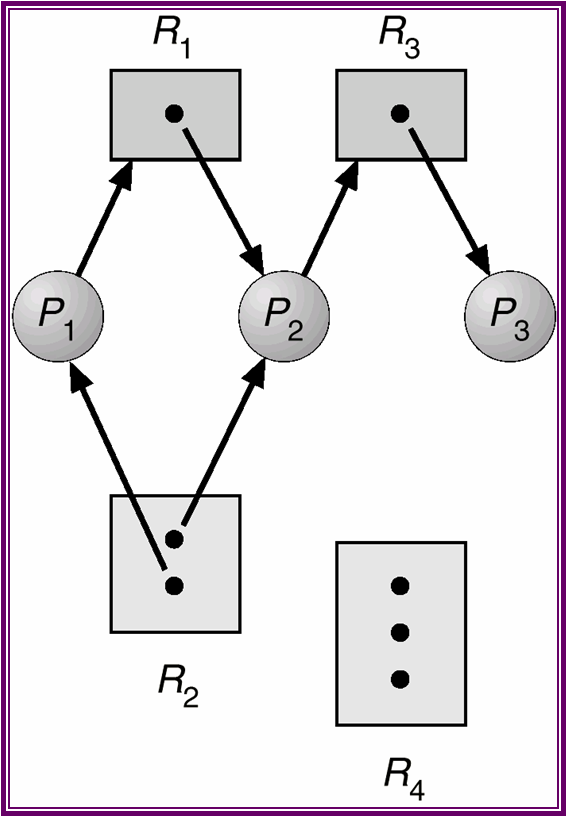
\includegraphics[scale=0.5]{v6f8-1}
  \end{center}
  \end{frame}

  %% PAGE
  \begin{frame}
  \frametitle{Deadlock and resource-allocation graph} \pause
  \begin{itemize}
  \item{Given the definition of a resource-allocation graph, it can be shown that} \pause
    \begin{itemize}
    \item{If the graph contains no cycles, then no process in the system is deadlocked;} \pause
    \item{If the graph does contain a cycle, then a deadlock \emph{may} exist.} \pause
    \end{itemize}
  \end{itemize}
  \begin{minipage}[c]{0.5\textwidth}
    \centering
    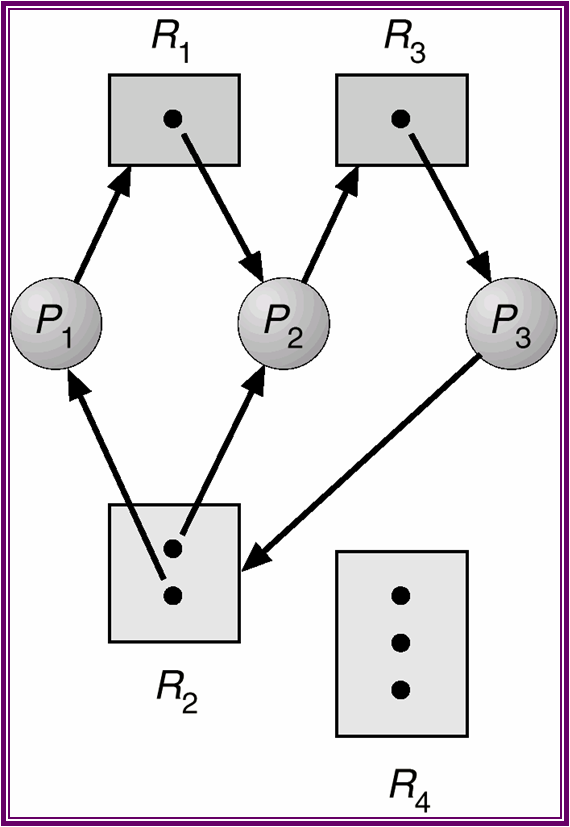
\includegraphics[scale=.3]{v6f8-2} \pause
    \newline Deadlocked \pause
  \end{minipage}%
  \begin{minipage}[c]{0.5\textwidth}
    \centering
    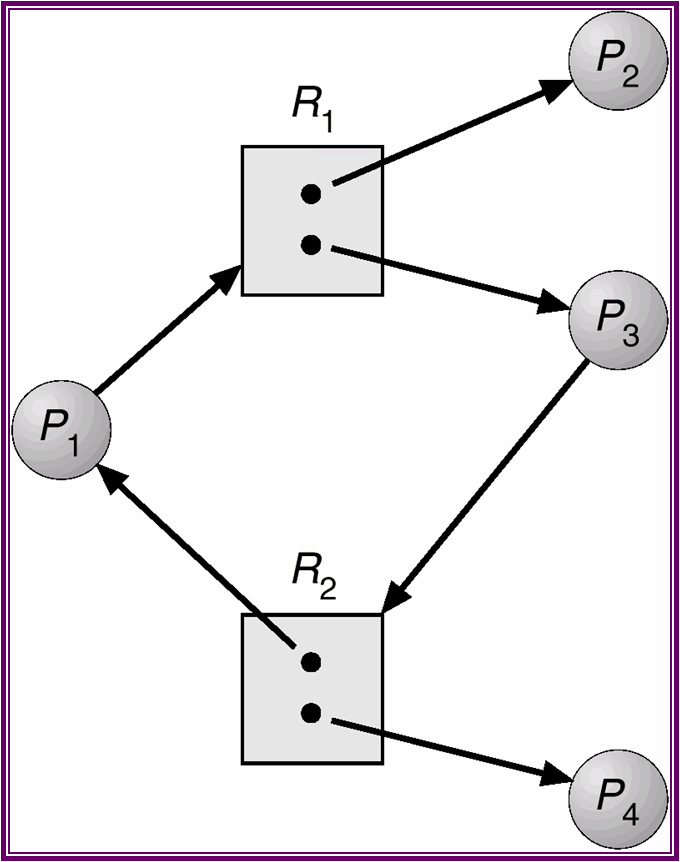
\includegraphics[scale=.3]{v6f8-3} \pause
    \newline Not deadlocked
  \end{minipage}
  \end{frame}

  %% PAGE
  \begin{frame}
  \frametitle{Questions}
    \begin{itemize}
	  \item{Any questions?}
    \end{itemize}
    \begin{center}
	  
\includegraphics[scale=.5]{question}
    \end{center}
  \end{frame}

\section{Methods of handling deadlock}

\subsection{Deadlock prevention}

  %% PAGE
  \begin{frame}
  \frametitle{Deadlock prevention (1/4)} \pause
  \begin{itemize}
  \item{As we know, all the four necessary conditions must hold for a deadlock to occur.} \pause
    \begin{itemize}
    \item{Deadlock can be prevented by attacking at least one of these conditions.} \pause
    \end{itemize}
  \item{Attacking ``mutual exclusion''} \pause
    \begin{itemize}
    \item{It's not required for sharable resources, such as read-only files; \pause It must hold for non-sharable resources, such as printer.} \pause
    \item{If a device (such as printer) can be spooled} \pause
      \begin{itemize}
      \item{Only the printer server uses printer resource (other processes send documents to the printer server to be printed), then deadlock for printer is eliminated.} \pause
      \item{But, not all devices can be spooled.} \pause
      \end{itemize}
    \item{In general, we cannot prevent deadlocks by attacking mutual exclusion: Some resources are intrinsically non-sharable.}
    \end{itemize}
  \end{itemize}
  \end{frame}

  %% PAGE
  \begin{frame}
  \frametitle{Deadlock prevention (2/4)} \pause
  \begin{itemize}
  \item{Attacking ``hold and wait''} \pause
    \begin{itemize}
    \item{We must guarantee that whenever a process requests a resource, it does not hold any other resources.} \pause
      \begin{itemize}
      \item{Require process to request and be allocated all its resources before it begins execution, \pause or allow process to request resources only when the process has none.} \pause
      \item{May result in low resource utilization and possible starvation.}
      \end{itemize}
    \end{itemize}
  \end{itemize}
  \end{frame}

  %% PAGE
  \begin{frame}
  \frametitle{Deadlock prevention (3/4)} \pause
  \begin{itemize}
  \item{Attacking ``no preemption''} \pause
    \begin{itemize}
    \item{If a process that is holding some resources requests another resource that cannot be immediately allocated to it, then all resources currently being held are released.} \pause
    \item{This can be applied to resources whose state can be easily saved and restored later, such as CPU.} \pause
      \begin{itemize}
      \item{It cannot generally be applied to to such resources as printers and tape drives.}
      \end{itemize}
    \end{itemize}
  \item{Attacking ``circular wait''} \pause
    \begin{itemize}
    \item{We can impose a total ordering of all resource types, and require that each process requests resources in an increasing order of enumeration.} \pause
    \end{itemize}
  \end{itemize}
  \end{frame}

\iffalse

  \begin{frame}
  \frametitle{Deadlock prevention (4/4)} \pause
  \begin{itemize}
  \item{Summary} \pause
    \newline
    \begin{center}
      \begin{tabular}{c|c}
        \textbf{Condition} & \textbf{Possible approach}\\
        \hline\hline \pause
        Mutual exclusion   & spool everything\\
        \hline \pause
        Hold and wait      & Request all resources initially\\
        \hline \pause
        No preemption      & Take resources away\\
        \hline \pause
        Circular wait      & Order resources numerically
      \end{tabular}
    \end{center}
  \end{itemize}
  \end{frame}

\fi

  %% PAGE
  \begin{frame}
  \frametitle{Questions}
  \begin{itemize}
  \item{Any questions?}
  \end{itemize}
  \begin{center}
    
\includegraphics[scale=.5]{question}
  \end{center}
  \end{frame}

\subsection{Deadlock avoidance}

  %% PAGE
  \begin{frame}
  \frametitle{Deadlock avoidance} \pause
  \begin{itemize}
  \item{Requires that the system has some additional \emph{a priori} information available.} \pause
    \begin{itemize}
    \item{Simplest and most useful model requires that each process declare the maximum number of resources of each type that it may need.} \pause
    \item{The deadlock-avoidance algorithm dynamically examines the resource-allocation state to ensure that there can never be a circular-wait condition.} \pause
      \begin{itemize}
      \item{Resource-allocation state is defined by the number of available and allocated resources, and the maximum demands of the processes.}
      \end{itemize}
    \end{itemize}
  \end{itemize}
  \end{frame}

  %% PAGE
  \begin{frame}
  \frametitle{Safe state (1/2)} \pause
  \begin{itemize}
  \item{When a process requests an available resource, system must decide if immediate allocation leaves the system in a \emph{safe state}.} \pause
    \begin{itemize}
    \item{System is in safe state if there exists a safe sequence of all processes $<P_0, P_1, ..., P_n>$ such that for each $P_i$, the resources that $P_i$ can still request can be satisfied by currently available resources plus resources held by all the $P_j$, with $j<i$.} \pause
    \end{itemize}
  \item{Basic facts} \pause
    \begin{itemize}
    \item{If a system is in safe state, no deadlocks;} \pause
    \item{If a system is in unsafe state,  possibility of deadlock.} \pause
    \end{itemize}
  \item{Deadlock avoidance must ensure that a system will never enter an unsafe state.}
  \end{itemize}
  \end{frame}

  %% PAGE
  \begin{frame}
  \frametitle{Safe state (2/2)} \pause
  \begin{center}
    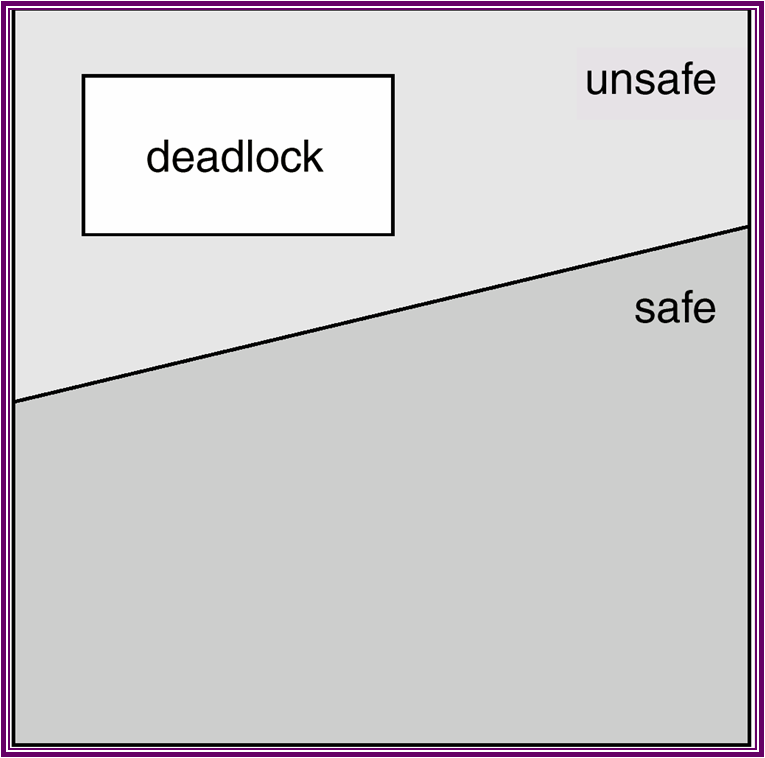
\includegraphics[scale=0.5]{v6f8-4}
  \end{center}
  \end{frame}

  %% PAGE
  \begin{frame}
  \frametitle{Banker's algorithm} \pause
  \begin{itemize}
  \item{Banker's algorithm} \pause
    \begin{itemize}
    \item{It's invented by Dijkstra in 1968 and used on the \textbf{THE} operating system.} \pause
    \item{It can be used in a banking system to ensure that the bank never allocates its available cash such that it can no longer satisfy the needs of all its customers.} \pause
    \end{itemize}
  \item{It requires that a new process must declare the maximum number of instances of each resource type that it may need.}
  \end{itemize}
  \end{frame}

  %% PAGE
  \begin{frame}
  \frametitle{Banker's algorithm: data structure} \pause
  \begin{itemize}
  \item{Data structures} \pause
    \begin{itemize}
    \item{$Available$:  Vector of length $m$. If $available[j] = k$, there are $k$ instances of resource type $R_j$ available.} \pause
    \item{Max: $n \times m$ matrix.  If $Max[i,j] = k$, then process $P_i$ may request at most $k$ instances of resource type $R_j$.} \pause
    \item{$Allocation$:  $n \times m$ matrix.  If $Allocation[i,j] = k$ then $P_i$ is currently allocated $k$ instances of $R_j$.} \pause
      \begin{itemize}
      \item{$Allocation_i$ means $i$th row of the $Allocation$.} \pause
      \end{itemize}
    \item{$Need$:  $n \times m$ matrix. If $Need[i,j] = k$, then $P_i$ may need $k$ more instances of $R_j$ to complete its task.} \pause
      \begin{itemize}
      \item{$Need[i,j] = Max[i,j] - Allocation [i,j]$.} \pause
      \item{$Need_i$ means $i$th row of the $Nead$.}
      \end{itemize}
    \end{itemize}
  \end{itemize}
  \end{frame}

  %% PAGE
  \begin{frame}
  \frametitle{Banker's algorithm: Safety detection} \pause
  \begin{enumerate}
  \item{Let $Work$ and $Finish$ be vectors of length $m$ and $n$, respectively. Initialize $Work = Available$ and $Finish[i] = false$, for $i=1, 2, ..., n$.} \pause
  \item{Find an $i$ such that \pause
      \newline
      $Finish[i] = false$ and $Need_i \leq Work$. \pause
      \newline
      If no such $i$ exists, go to step 4. \pause
    }
  \item{$Work = Work + Allocation_i$; $Finish[i] = true$; \newline go to step 2.} \pause
  \item{If $Finish[i] = true$ for all $i$, then the system is in a safe state.} \pause
  \end{enumerate}
  \begin{itemize}
  \item{This algorithm requires an order of $m \times n^2$ operations for safety detection.}
  \end{itemize}
  \end{frame}

  %% PAGE
  \begin{frame}
  \frametitle{Banker's algorithm: Resource-request (1/2)} \pause
  \begin{itemize}
  \item{Let $Request_i$ be the request vector for process $P_i$. } \pause
    \begin{itemize}
    \item{If $Request_i[j] = k$ then process $P_i$ wants $k$ instances of resource type $R_j$.}
    \end{itemize}
  \end{itemize}
  \end{frame}

  %% PAGE
  \begin{frame}
  \frametitle{Banker's algorithm: Resource-request (2/2)} \pause
  \begin{enumerate}
  \item{If $Request_i \leq Need_i$, go to step 2. Otherwise, raise error condition, since process has exceeded its maximum claim.} \pause
  \item{If $Request_i \leq Available$, go to step 3.  Otherwise $P_i$ must wait, since resources are not available.} \pause
  \item{Pretend to allocate requested resources to $P_i$ by modifying the state as follows: \newline \pause
      $Available = Available - Request_i;$ \newline \pause
      $Allocation_i = Allocation_i + Request_i;$ \newline \pause
      $Need_i = Need_i - Request_i;$ \newline \pause
    }
  \item{If the system is in safe state, the resources are allocated to $P_i$; \newline \pause
      Otherwise $P_i$ must wait, and the old resource-allocation state is restored.
    }
  \end{enumerate}
  \end{frame}

  %% PAGE
  \begin{frame}
  \frametitle{Banker's algorithm: example (1/3)} \pause
  \begin{itemize}
  \item{5 processes and 3 resource types} \pause
    \begin{itemize}
    \item{Type A has 10 instance, B has 5 and C has 7.} \pause
    \end{itemize}
  \item{Snapshot at time $T_0$:} \pause
  \end{itemize}
  \begin{tabular}{cccc}
    Process & Max   & Allocation & Available\\
    \hline
            & A B C & A B C      & A B C\\
    $P_0$   & 7 5 3 & 0 1 0      & 3 3 2\\
    $P_1$   & 3 2 2 & 2 0 0      &      \\
    $P_2$   & 9 0 2 & 3 0 2      &      \\
    $P_3$   & 2 2 2 & 2 1 1      &      \\
    $P_4$   & 4 3 3 & 0 0 2      &      \\
  \end{tabular}
  \end{frame}

  %% PAGE
  \begin{frame}
  \frametitle{Banker's algorithm: example (2/3)} \pause
  \begin{itemize}
  \item{The content of the matrix $Need$ is defined to be $Max - Allocation$.} \pause
  \end{itemize}
  \begin{tabular}{cc}
    Process & Need\\
    \hline
            & A B C\\
    $P_0$   & 7 4 3\\
    $P_1$   & 1 2 2\\
    $P_2$   & 6 0 0\\
    $P_3$   & 0 1 1\\
    $P_4$   & 4 3 1\\
  \end{tabular} \pause
  \begin{itemize}
  \item{The system is in a safe state since the sequence $<P_1, P_3, P_4, P_2, P_0>$ satisfies safety criteria.}
  \end{itemize}
  \end{frame}

  %% PAGE
  \begin{frame}
  \frametitle{Banker's algorithm: example (3/3)} \pause
  \begin{itemize}
  \item{Assume that $P_1$ further requests (1, 0, 2) ($\leq$(3,3,2))} \pause
  \end{itemize}
  \begin{tabular}{ccccc}
    Process & Max   & Allocation & Need  & Available\\
    \hline
            & A B C & A B C      & A B C & A B C\\
    $P_0$   & 7 5 3 & 0 1 0      & 7 4 3 & 2 3 0\\
    $P_1$   & 3 2 2 & 3 0 3      & 0 2 0 &      \\
    $P_2$   & 9 0 2 & 3 0 2      & 6 0 0 &      \\
    $P_3$   & 2 2 2 & 2 1 1      & 0 1 1 &      \\
    $P_4$   & 4 3 3 & 0 0 2      & 4 3 1 &      \\
  \end{tabular} \pause
  \begin{itemize}
  \item{Executing safety algorithm shows that sequence $<P_1, P_3, P_4, P_0, P_2>$ satisfies safety requirement.} \pause
    \begin{itemize}
    \item{Can request for (3,3,0) by $P_4$ be granted?} \pause
      % \begin{itemize}
      % \item{No, since the resources are not available.} \pause
      % \end{itemize}
    \item{Can request for (0,2,0) by $P_0$ be granted?}
      % \begin{itemize}
      % \item{No, since the resulting state is unsafe} \pause
      % \end{itemize}
    \end{itemize}
  \end{itemize}
  \end{frame}

  %% PAGE
  \begin{frame}
  \frametitle{Questions}
  \begin{itemize}
  \item{Any questions?}
  \end{itemize}
  \begin{center}
    
\includegraphics[scale=.5]{question}
  \end{center}
  \end{frame}

\subsection{Deadlock detection and recovery}

  %% PAGE
  \begin{frame}
  \frametitle{Deadlock detection and recovery} \pause
  \begin{itemize}
  \item{If a system does not employ either a deadlock-prevention or a deadlock-avoidance algorithm, then a deadlock situation may occur.} \pause
  \item{In this situation, the operating system must provide:} \pause
    \begin{itemize}
    \item{An algorithm to determine whether a deadlock has occurred;} \pause
    \item{An algorithm to recover from the deadlock.}
    \end{itemize}
  \end{itemize}
  \end{frame}

  %% PAGE
  \begin{frame}
  \frametitle{Deadlock detection algorithm} \pause
  \begin{enumerate}
  \item{Let $Work$ and $Finish$ be vectors of length $m$ and $n$, respectively.\newline \pause Initialize $Work = Available$ and if $Allocation_i \neq 0$, then $Finish[i] = false$;otherwise, $Finish[i] = true$.} \pause
  \item{Find an index $i$ such that \newline \pause
      $Finish[i] = false$ and $Request_i \leq Work$ \newline \pause
      If no such $i$ exists, go to step 4. } \pause
  \item{$Work = Work + Allocation_i$; $Finish[i] = true$; \newline go to step 2.} \pause
  \item{If $Finish[i] = false$ for some $i$ ($1 \leq i \leq n$), then the system is in deadlock state.} \pause
    \begin{itemize}
    \item{$P_i$ is deadlocked if $Finish[i] = false$.}
    \end{itemize}
  \end{enumerate}
  \end{frame}

  %% PAGE
  \begin{frame}
  \frametitle{Deadlock detection algorithm: example (1/2)} \pause
  \begin{itemize}
  \item{5 processes and 3 resource types} \pause
    \begin{itemize}
    \item{Type A has 7 instance, B has 2 and C has 6.} \pause
    \end{itemize}
  \item{Snapshot at time $T_0$:} \pause
  \end{itemize}
  \begin{tabular}{cccc}
    Process & Allocation & Request & Available\\
    \hline
            & A B C      & A B C   & A B C\\
    $P_0$   & 0 1 0      & 0 0 0   & 0 0 0\\
    $P_1$   & 2 0 0      & 2 0 2   &      \\
    $P_2$   & 3 0 3      & 0 0 0   &      \\
    $P_3$   & 2 1 1      & 1 0 0   &      \\
    $P_4$   & 0 0 2      & 0 0 2   &      \\
  \end{tabular} \pause
  \begin{itemize}
  \item{Sequence $<P_0, P_2, P_3, P_1, P_4>$ will result in $Finish[i] = true$ for all $i$.}
  \end{itemize}
  \end{frame}

  %% PAGE
  \begin{frame}
  \frametitle{Deadlock detection algorithm: example (2/2)} \pause
  \begin{itemize}
  \item{Suppose $P_2$ further requests an additional instance of type C.} \pause
  \end{itemize}
  \begin{tabular}{cc}
    Process & Request\\
    \hline
            & A B C\\
    $P_0$   & 0 0 0\\
    $P_1$   & 2 0 1\\
    $P_2$   & 0 0 1\\
    $P_3$   & 1 0 0\\
    $P_4$   & 0 0 2\\
  \end{tabular} \pause
  \begin{itemize}
  \item{State of the system?} \pause
    \begin{itemize}
    \item{Deadlock exists, consisting of processes $P_1$,  $P_2$, $P_3$, and $P_4$.}
    \end{itemize}
  \end{itemize}
  \end{frame}

  %% PAGE
  \begin{frame}
  \frametitle{Deadlock detection algorithm: Usage} \pause
  \begin{itemize}
  \item{When and how often to invoke deadlock detection algorithm depends on} \pause
    \begin{enumerate}
    \item{How often is a deadlock likely to occur?} \pause
    \item{How many processes will be affected by deadlock when it happens?}
    \end{enumerate}
  \end{itemize}
  \end{frame}

  %% PAGE
  \begin{frame}
  \frametitle{Questions}
  \begin{itemize}
  \item{Any questions?}
  \end{itemize}
  \begin{center}
    
\includegraphics[scale=.5]{question}
  \end{center}
  \end{frame}

  %% PAGE
  \begin{frame}
  \frametitle{Recovery from deadlock} \pause
  \begin{itemize}
  \item{When a detection algorithm determines that a deadlock exists, two options are available.} \pause
    \begin{enumerate}
    \item{Process termination} \pause
      \begin{itemize}
      \item{Abort all deadlocked processes} \pause
      \item{Abort one process at a time until the deadlock cycle is eliminated.} \pause
      \end{itemize}
    \item{Resource preemption} \pause
%      \begin{itemize}
%      \item{Select a victim.} \pause
%      \item{Rollback} \pause
%      \item{Starvation} \pause
%      \end{itemize}
    \end{enumerate}
  \item{Both of them are NOT easy.}
  \end{itemize}
  \end{frame}

  %% PAGE
  \begin{frame}
  \frametitle{Questions}
  \begin{itemize}
  \item{Any questions?}
  \end{itemize}
  \begin{center}
    
\includegraphics[scale=.5]{question}
  \end{center}
  \end{frame}

  \subsection{Ostrich algorithm}

  %% PAGE
  \begin{frame}
  \frametitle{Ostrich algorithm} \pause
  \begin{itemize}
	%\item{We can design a protocol to prevent or avoid deadlocks, ensuring that the system will \emph{never} enter a deadlock state;} \pause
	%\item{We can allow the system to enter a deadlock state, detect it, and recover from it;} \pause
	\item{We can ignore the problem altogether, and pretend that deadlocks never occur in the system.} \pause
	\begin{itemize}
		\item{This solution is used by \emph{most} operating systems, including Windows and Unix/Linux.} \pause
		\item{Because the deadlocks occur very rarely and the deadlock-prevention, deadlock-avoidance or deadlock-detection and recovery algorithms are \emph{costly}.} \pause
		\item{It's a trade-off between \emph{convenience} and \emph{correctness}.}
	\end{itemize}
  \end{itemize}
  \end{frame}

  %% PAGE
  \begin{frame}
  \frametitle{Questions}
  \begin{itemize}
	\item{Any questions?}
  \end{itemize}
  \begin{center}
	
\includegraphics[scale=.5]{question}
\end{center}
\end{frame}

  %% PAGE
\end{CJK*}
\end{document}
